% Recovered verbatim from the six-page report/report.pdf at GitHub commit
% 8d6669b4b5c3078718dd6d3e058641a85b64f303. The supplied ZIP is an earlier draft.
% Figure pixels are extracted directly from the original PDF, without redrawing.
\documentclass[10pt,twocolumn,a4paper]{article}
\usepackage[utf8]{inputenc}
\usepackage[T1]{fontenc}
\usepackage{amsmath,amssymb,amsthm}
\usepackage{mathtools}
\usepackage{algorithm}
\usepackage{algpseudocode}
\usepackage[margin=1.8cm,top=2cm,bottom=2cm]{geometry}
\usepackage{parskip}
\usepackage{abstract}
\usepackage{enumitem}
\usepackage{hyperref}
\usepackage[authoryear]{natbib}
\setcitestyle{square}
\usepackage{subcaption}
\usepackage{graphicx}
\usepackage{booktabs}
\hypersetup{colorlinks=true,linkcolor=black,citecolor=black,urlcolor=black}
\newcommand{\statespace}{\mathcal{S}}
\newcommand{\board}{\mathcal{B}}
\newcommand{\bigO}{\mathcal{O}}
\theoremstyle{definition}
\newtheorem{definition}{Definition}[section]
\newtheorem{example}{Example}[section]
\newtheorem{proposition}{Proposition}[section]
\theoremstyle{remark}
\newtheorem{remark}{Remark}[section]
\title{\textbf{Solving the 3D $N^2$ Queens Problem\\ via Markov Chain Monte Carlo}}
\author{Chengheng Li Chen, Francisco Badia Laguillo, Jacopo Senoner\\
\textit{School of Computer and Communication Sciences}\\
\textit{EPFL, Lausanne, Switzerland}\\
\texttt{\{chengheng.lichen, francisco.badialaguillo, jacopo.senoner\}@epfl.ch}}
\date{}
\begin{document}
\maketitle

\begin{abstract}
The classical $N$-queens problem admits a natural three-dimensional generalization: placing $N^2$ mutually non-attacking queens on an $N\times N\times N$ cubic board, where queens attack along rook lines, planar diagonals, and space diagonals. We formulate this as energy minimization and develop a Metropolis-Hastings algorithm with simulated annealing, proving correctness by establishing irreducibility, aperiodicity, and weak reversibility. Experiments for $N=3$ to $N=11$ confirm theoretical predictions: instances with $\gcd(N,210)>1$ converge to positive energy, while $N=11$ reaches zero-energy configurations. We find that only the linear energy transformation reliably attains global minima, and that constant high-$\beta$ schedules suffice for moderate $N$, suggesting a benign energy landscape at these problem sizes.
\end{abstract}

\section{Introduction}
The classical $N$-queens problem asks to place $N$ queens on an $N\times N$ chessboard such that no two queens attack each other. This work studies a natural three-dimensional generalization: placing $N^2$ queens on an $N\times N\times N$ cubic board without mutual attacks.

The transition to three dimensions introduces additional attack directions and a substantially larger configuration space, rendering exhaustive enumeration infeasible for moderate values of $N$. We therefore adopt a Markov Chain Monte Carlo (MCMC) approach, constructing a Markov chain whose stationary distribution concentrates on low-energy configurations.

The remainder of this report is organized as follows. Section~\ref{sec:formulation} formalizes the problem by introducing the attack relations, state space, and energy function, addressing the first two questions of the mini-project description. Section~\ref{sec:mcmc} develops the MCMC algorithm and discusses the design of the proposal distribution, addressing the remaining question of Section~2. Section~\ref{sec:experiments} presents experimental results, with each subsection corresponding to a question from the mini-project description. Section~\ref{sec:conclusion} offers concluding remarks.

\section{Problem Formulation}\label{sec:formulation}
We begin by establishing the mathematical framework for the three-dimensional queens problem.

\subsection{Board and Positions}
\begin{definition}[Board]
The \emph{board} is the discrete cube $\board_N=\{0,1,\ldots,N-1\}^3$. Each element $(i,j,k)\in\board_N$ represents a \emph{position}, where $i$, $j$, and $k$ denote coordinates along the three orthogonal axes.
\end{definition}
For instance, when $N=4$, the board contains $4^3=64$ positions, and we seek to place $4^2=16$ queens.

\subsection{Attack Relations}
In three dimensions, queens attack along more directions than in the classical planar setting. We identify three distinct types of attack, each generalizing a familiar movement pattern from two-dimensional chess.

\begin{definition}[Attack Relation]\label{def:attack}
Two distinct positions $(i,j,k)$ and $(i',j',k')$ are said to be \emph{in attack} if any of the following conditions holds:
\begin{itemize}[leftmargin=*]
\item \textbf{Rook-type attack:} The positions share at least two coordinates. Equivalently, they have the same pair $(i,j)$, the same pair $(i,k)$, or the same pair $(j,k)$.
\item \textbf{Planar diagonal attack:} The positions lie on a common diagonal within one of the three coordinate planes. In the $xy$-plane (when $k=k'$), this occurs when $|i-i'|=|j-j'|\ne0$. Analogous conditions apply to the $xz$-plane and the $yz$-plane.
\item \textbf{Space diagonal attack:} All three coordinate differences have equal nonzero magnitude: $|i-i'|=|j-j'|=|k-k'|\ne0$.
\end{itemize}
\end{definition}
The rook-type and planar diagonal attacks generalize the movement of the ``classical'' chess queen to each axis-aligned plane. The space diagonal condition introduces the four families of diagonals that traverse the interior of the cube, a feature unique to three dimensions.

\begin{example}[Central Queen]
On a $3\times3\times3$ board, a queen at $(1,1,1)$ attacks $(0,0,0)$ and $(2,2,2)$ via space diagonals, $(0,1,1)$ and $(2,1,1)$ via rook-type (shared $j,k$), and $(0,0,1)$ and $(2,2,1)$ via planar diagonals in the $k=1$ plane.
\end{example}

\begin{example}[Non-Attacking Pair]
Queens at $(0,0,0)$ and $(2,1,3)$ do not attack: no two coordinates match (not rook-type), coordinate differences $2,1,3$ are pairwise distinct (not planar), and not all equal (not space diagonal).
\end{example}

\subsection{State Space}
We now define how configurations of queens are represented. Since queens are indistinguishable, two arrangements occupying the same set of positions are considered identical.

\begin{definition}[Configuration and State Space]
A \emph{configuration} is a set $s\subset\board_N$ of $N^2$ distinct positions. The \emph{state space} is
\[
\statespace=\bigl\{s\subset\board_N:|s|=N^2\bigr\},
\]
with cardinality $|\statespace|=\binom{N^3}{N^2}$.
\end{definition}
This general formulation admits any arrangement of $N^2$ queens on the board. For $N=3$, we have $|\statespace|=\binom{27}{9}\approx4.7\times10^6$ configurations, and for $N=4$, this grows to $|\statespace|\approx4.9\times10^{13}$, rendering exhaustive search infeasible.

\subsubsection{Possible State Space Reductions}
Several approaches can reduce the effective size of the state space.

\textbf{Restricted configurations.} Rather than representing a configuration as an arbitrary set of $N^2$ positions, one can encode it as a function $\kappa:\{0,\ldots,N-1\}^2\to\{0,\ldots,N-1\}$, placing exactly one queen at position $(i,j,\kappa(i,j))$ for each pair $(i,j)$. Geometrically, this places one queen per vertical line parallel to the $k$-axis. The restricted state space has cardinality $N^{N^2}$, substantially smaller than $\binom{N^3}{N^2}$. Moreover, rook-type attacks along the $k$-axis are eliminated by construction, since no two queens can share the same $(i,j)$ coordinates. Importantly, this restriction preserves all zero-energy solutions: any valid solution must have exactly one queen per $(i,j)$ pair, as having two would create a rook-type attack.

\textbf{Symmetry reduction.} The cubic board $\board_N$ admits geometric symmetries including rotations and reflections. These symmetries partition the state space into equivalence classes, and one could in principle explore only one representative per class. However, this approach is not effective for MCMC: all configurations in the same equivalence class share the same energy, so the algorithm already treats them equivalently. Furthermore, computing the canonical representative of an equivalence class is computationally costly, adding overhead without improving convergence.

For simplicity of implementation, we adopted the general state space $\statespace$ without these reductions in our experiments. The MCMC algorithm remains correct on the full space, and the moderate values of $N$ considered did not require additional optimizations.

\subsection{Energy Function}\label{subsec:energy}
The energy function quantifies the degree of conflict in a configuration. A valid solution, in which no two queens attack each other, corresponds to zero energy.

\begin{definition}[Energy Function]\label{def:energy}
The \emph{energy} of a configuration $s\in\statespace$ is the number of attacking pairs:
\begin{equation}
J(s):=\sum_{\{q,q'\}\subseteq s}\mathbf{1}\bigl[q\text{ attacks }q'\bigr].
\end{equation}
\end{definition}
The energy counts unordered pairs of mutually attacking queens, rather than the number of endangered queens. Each attacking pair is counted exactly once, even if the two queens attack each other along multiple directions simultaneously. Thus $J(s)=0$ if and only if no attacks exist.

Second, the function $g$ offers flexibility in shaping the energy landscape:
\begin{itemize}[leftmargin=*]
\item $g(x)=x$: directly counts attacking pairs (our choice).
\item $g(x)=x^2$: penalizes high-conflict states more heavily.
\item $g(x)=\log(1+x)$: compresses large values.
\end{itemize}

\begin{example}[Energy Calculation]
For $N=2$, consider four queens at $(0,0,0)$, $(0,0,1)$, $(1,1,0)$, $(1,1,1)$. The pairs $\{(0,0,0),(0,0,1)\}$ and $\{(1,1,0),(1,1,1)\}$ each share two coordinates (rook-type attacks), so $J(s)=2$.
\end{example}

\subsubsection{Energy Computation}
A direct approach to computing $J(s)$ examines all $\binom{N^2}{2}$ pairs of queens and checks whether each pair satisfies any of the attack conditions in Definition~\ref{def:attack}. This yields $\bigO(N^4)$ complexity.

\begin{algorithm}[H]
\caption{Direct Energy Computation}
\begin{algorithmic}[1]
\Require Configuration $s=\{q_0,\ldots,q_{N^2-1}\}$
\Ensure Energy $J(s)$
\State $\mathrm{count}\gets0$
\For{$i=0$ to $N^2-1$}
\For{$j=i+1$ to $N^2-1$}
\If{\Call{CheckAttack}{$q_i,q_j$}}
\State $\mathrm{count}\gets\mathrm{count}+1$
\EndIf
\EndFor
\EndFor
\State \Return $\mathrm{count}$
\end{algorithmic}
\end{algorithm}

\begin{remark}[Attack Check]
The function \textsc{CheckAttack}$(q,q')$ returns true if positions $q=(i,j,k)$ and $q'=(i',j',k')$ satisfy any attack condition: rook-type (sharing two coordinates), planar diagonal ($|i-i'|=|j-j'|$ with $k=k'$, or analogously for other planes), or space diagonal ($|i-i'|=|j-j'|=|k-k'|\ne0$). Each check requires $\bigO(1)$ time.
\end{remark}

Note that two queens may attack each other through multiple attack types simultaneously. For instance, queens at $(0,0,0)$ and $(1,1,0)$ attack via both rook-type (shared $k$) and planar diagonal (in the $k=0$ plane). However, this pair contributes only one conflict to the energy, as we count attacking pairs rather than attack relationships.

\begin{remark}[Incremental Updates]
When a single queen moves from position $q$ to position $q'$, the energy change $\Delta J$ can be computed in $\bigO(N^2)$ time by checking the moved queen against all $N^2-1$ other queens.
\end{remark}

An alternative approach maintains counts of queens on each of the 13 attack line families, enabling $\bigO(1)$ incremental updates. However, this method counts attack relationships rather than attacking pairs, overcounting when two queens attack via multiple lines. For the moderate values of $N$ in our experiments, the direct algorithm provided sufficient performance, and we adopted it for simplicity and correctness.

\section{MCMC Algorithm}\label{sec:mcmc}
We cast the search for a zero-energy configuration as a sampling problem. The Metropolis-Hastings algorithm generates a Markov chain whose stationary distribution concentrates probability on low-energy states. By gradually lowering the temperature, the chain is guided toward configurations of minimal energy.

\subsection{Proposal Base Chain}
The proposal base chain defines how candidate moves are generated. Let $\Psi=(\psi_{ss'})$ denote its transition matrix. For the Metropolis-Hastings algorithm to converge to the correct stationary distribution, the proposal chain must be irreducible (any configuration reachable from any other), aperiodic (no deterministic cycling), and weakly reversible ($\psi_{ss'}>0$ if and only if $\psi_{s's}>0$). The last condition ensures that the Metropolis-Hastings chain satisfies detailed balance with respect to the target distribution.

We adopt a single-queen move that satisfies all three conditions.

\begin{definition}[Move Proposal]
Given a configuration $s\in\statespace$, a new configuration $s'$ is proposed by selecting a queen $q\in s$ uniformly at random, selecting an empty cell $q'\in\board_N\setminus s$ uniformly at random, and defining $s':=(s\setminus\{q\})\cup\{q'\}$.
\end{definition}
The proposal probability from $s$ to $s'$ is $\psi_{ss'}=\frac{1}{N^2}\cdot\frac{1}{N^3-N^2}$, since we select uniformly among $N^2$ queens and $N^3-N^2$ empty cells.

\begin{proposition}[Correctness of the Proposal Chain]
The proposal chain is irreducible, aperiodic, and weakly reversible on $\statespace$.
\end{proposition}
\begin{proof}
For irreducibility, observe that any configuration $s$ can be transformed into any other configuration $s'$ through a finite sequence of single-queen moves: we relocate each queen in $s\setminus s'$ to a temporary position, then move queens to their target positions in $s'\setminus s$. Since $|s|=|s'|=N^2$ and each move has positive probability, any two configurations communicate.

For aperiodicity, note that proposed moves are accepted with probability less than one when the energy increases, creating self-loops that prevent deterministic cycling.

For weak reversibility, suppose $s$ and $s'$ differ by moving queen $q$ to position $q'$, so that $s'=(s\setminus\{q\})\cup\{q'\}$. Then $\psi_{ss'}>0$ since $q\in s$ and $q'\notin s$. Symmetrically, $\psi_{s's}>0$ since $q'\in s'$ and $q\notin s'$. Thus $\psi_{ss'}>0$ if and only if $\psi_{s's}>0$.
\end{proof}

\begin{example}[Move Proposal]
For $N=3$ with a configuration $s$ containing 9 queens including one at $(0,0,0)$, suppose we select $q=(0,0,0)$ and empty cell $q'=(2,0,1)$. The proposed configuration is $s'=(s\setminus\{(0,0,0)\})\cup\{(2,0,1)\}$.
\end{example}

\begin{remark}[Choice of Move Size]
Allowing multiple queens to move simultaneously would increase connectivity but make transitions more random, reducing the effectiveness of gradual cooling. A single-queen move balances local refinement with global exploration when combined with simulated annealing.
\end{remark}

\subsection{Metropolis-Hastings Acceptance}
Given a proposal from configuration $s$ to $s'$, the Metropolis-Hastings algorithm accepts or rejects the move according to a probability that depends on the energy difference. This mechanism ensures that the chain satisfies detailed balance and converges to the desired stationary distribution.

\begin{definition}[Acceptance Probability]
The acceptance probability for a proposed move from $s$ to $s'$ is
\begin{equation}
a_{ss'}:=\begin{cases}
\min\bigl(1,\exp(-\beta\Delta J)\bigr)&\text{if }\psi_{ss'}>0,\\
0&\text{otherwise},
\end{cases}
\end{equation}
where $\Delta J=J(s')-J(s)$ denotes the energy difference and $\beta\ge0$ is the inverse temperature parameter.
\end{definition}
When $\Delta J\le0$, the proposed configuration has equal or lower energy, and the move is always accepted. When $\Delta J>0$, the move increases energy and is accepted with probability $\exp(-\beta\Delta J)$, which decreases as $\beta$ increases. This allows occasional uphill moves that help the chain escape local minima, with the frequency of such moves controlled by the temperature.

\begin{example}[Acceptance Decision]
Suppose $\beta=2$, $J(s)=5$, and $J(s')=7$, so $\Delta J=2$. The acceptance probability is $a_{ss'}=\exp(-2\cdot2)=e^{-4}\approx0.018$. Despite increasing energy, the move has a small chance of acceptance, allowing the chain to explore beyond local minima.
\end{example}

\subsection{Simulated Annealing}
Rather than fixing $\beta$ throughout the simulation, we allow it to vary over time according to a predefined schedule.

\begin{definition}[Annealing Schedule]
An annealing schedule specifies the inverse temperature $\beta^{(t)}$ at each step $t\in\{0,1,\ldots,T\}$, where $T$ is the total number of steps. The schedule interpolates from an initial value $\beta^{(0)}$ to a final value $\beta^{(T)}$.
\end{definition}
We consider two annealing schedules. The linear schedule increases $\beta$ at a constant rate:
\begin{equation}
\beta^{(t)}:=\beta^{(0)}+\left(\beta^{(T)}-\beta^{(0)}\right)\cdot\frac{t}{T}.
\end{equation}
The exponential schedule increases $\beta$ geometrically, spending more iterations at lower temperatures:
\begin{equation}
\beta^{(t)}:=\beta^{(0)}\cdot\left(\frac{\beta^{(T)}}{\beta^{(0)}}\right)^{t/T}.
\end{equation}

\begin{remark}[Schedule Comparison]
The linear schedule provides uniform coverage across temperature ranges, while the exponential schedule allocates more steps to the high-temperature regime, potentially improving exploration before the final cooling phase. The choice of schedule can significantly affect convergence behavior, as we investigate in Section~\ref{sec:experiments}.
\end{remark}

\section{Experimental Results}\label{sec:experiments}
We evaluate the MCMC algorithm for board sizes $N=4$ to $N=11$. A sufficient condition for the existence of a zero-energy configuration is $\gcd(N,210)=1$, conjectured to be necessary~\citep{Kunt2024nQueensHigherDimensions}. Values $N\in\{2,\ldots,10\}$ are proven unsolvable, while $N=11$ admits solutions. Thus, for $N\le10$ we expect convergence to positive energy, whereas for $N=11$ zero energy should be attainable.

All experiments average energy over multiple independent runs with distinct random seeds.

\subsection{Choice of Energy Transformation}
We compare the three transformations introduced in Section~\ref{subsec:energy} for $N=11$. As shown in Figure~\ref{fig:energy-transform}(a), linear and quadratic transformations both converge, while the logarithmic transformation oscillates without settling. Even with a substantially larger inverse temperature range ($\beta:50\to10000$), the logarithmic case converges only to a local minimum with final energy around 103 (Figure~\ref{fig:energy-transform}(b)), as the compression of energy differences flattens the landscape and traps the chain in suboptimal configurations. The quadratic transformation converges faster than linear but similarly fails to reach the global minimum consistently. Only the linear transformation reliably attains zero energy, and we therefore adopt $g(x)=x$ for all subsequent experiments.

\begin{figure}[t]
\centering
\begin{subfigure}{0.48\linewidth}
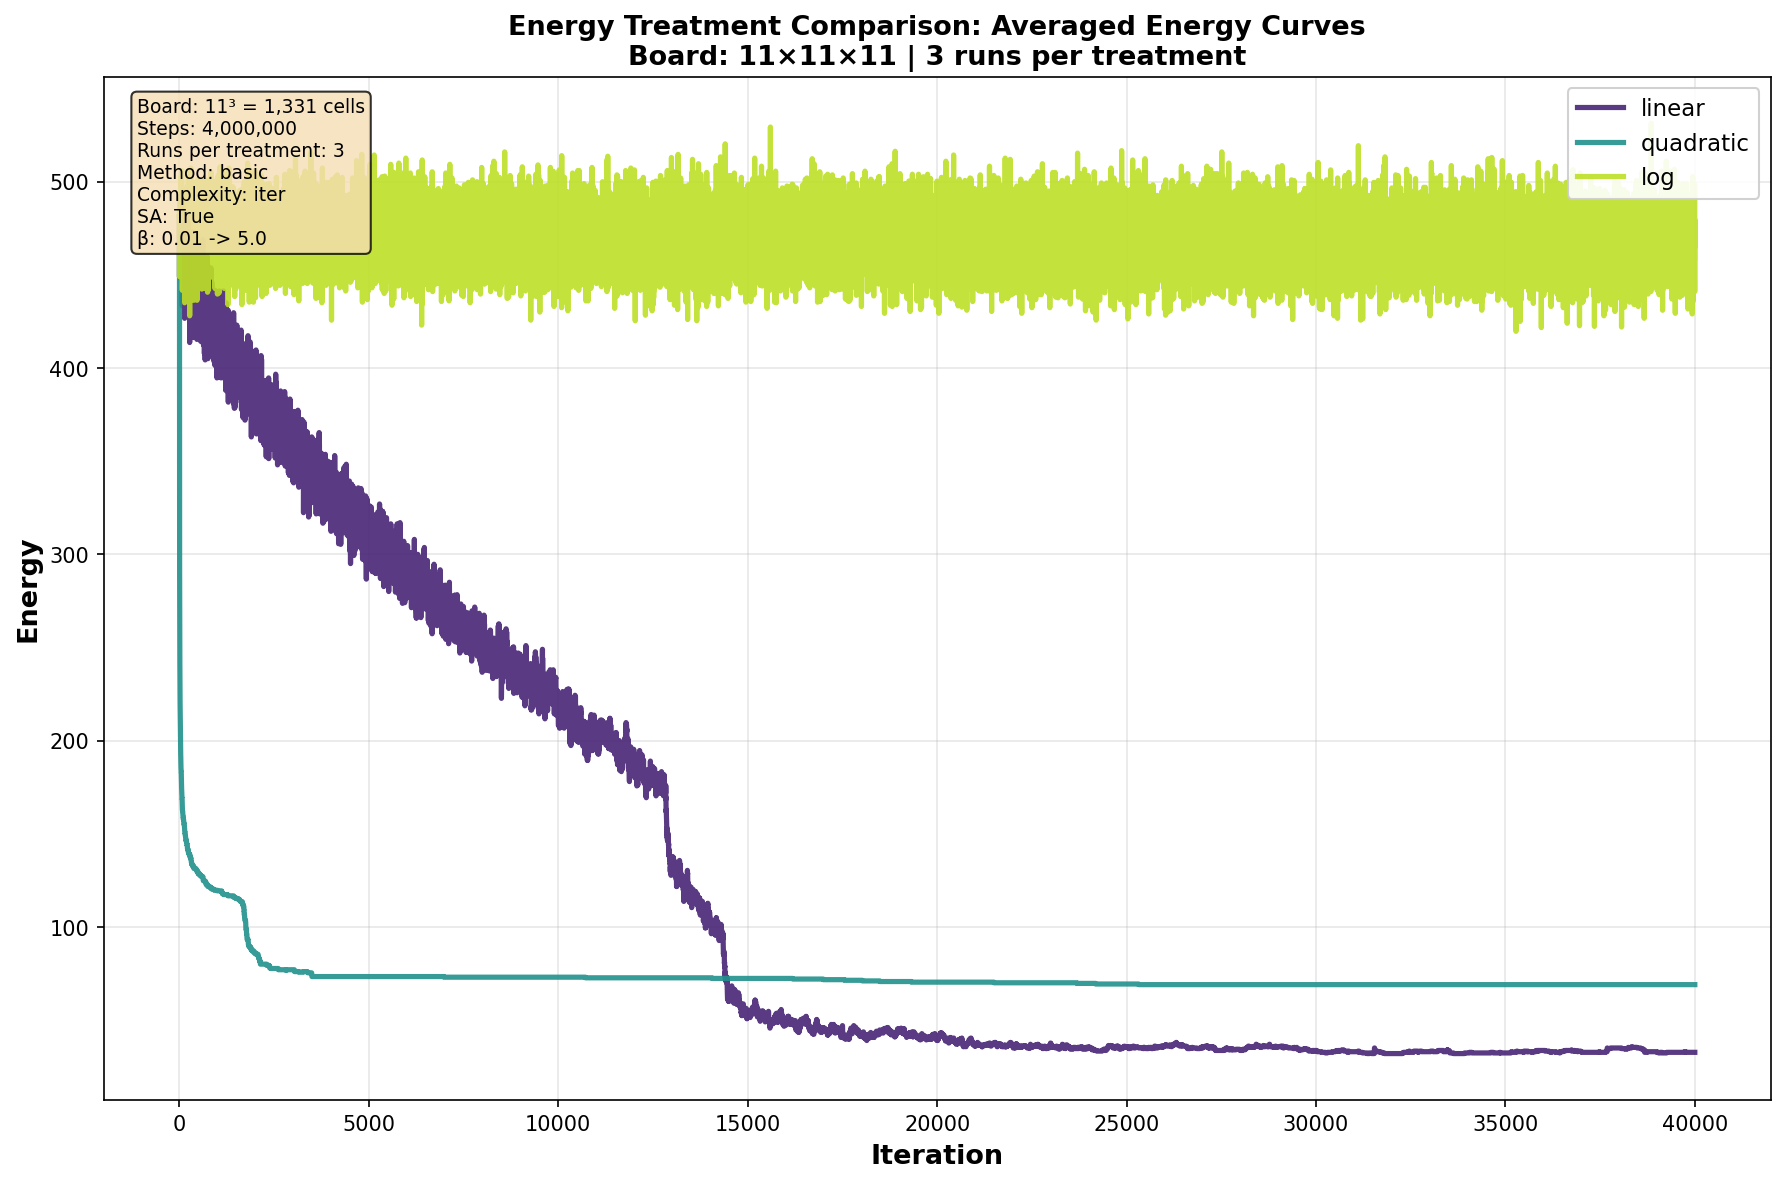
\includegraphics[width=\linewidth]{figures/energy-transform-comparison.png}
\caption{$g_1(x)=x$, $g_2(x)=x^2$, $g_3(x)=\log(x)$}
\end{subfigure}\hfill
\begin{subfigure}{0.48\linewidth}
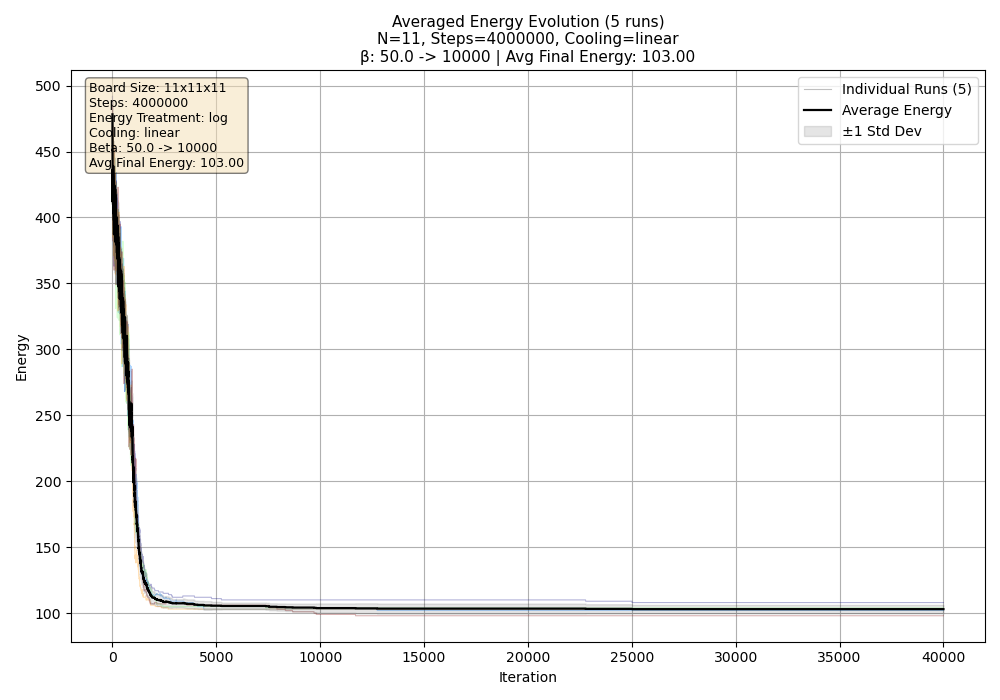
\includegraphics[width=\linewidth]{figures/energy-log-high-beta.png}
\caption{$g(x)=\log(x)$ with $\beta:50\to10000$}
\end{subfigure}
\caption{Energy evolution for $N=11$. (a) Logarithmic oscillates; linear and quadratic reach zero. (b) Larger $\beta$ enables logarithmic convergence, but only to a local minimum.}
\label{fig:energy-transform}
\end{figure}

\subsubsection{Non-Uniqueness of Solutions}
When zero-energy configurations exist, they are generally not unique. Figure~\ref{fig:solutions} displays two distinct solutions for $N=11$ obtained with different $g$ functions, represented as Latin squares where cell $(i,j)$ contains the queen's height $k$.

\begin{figure}[t]
\centering
\begin{subfigure}{0.48\linewidth}
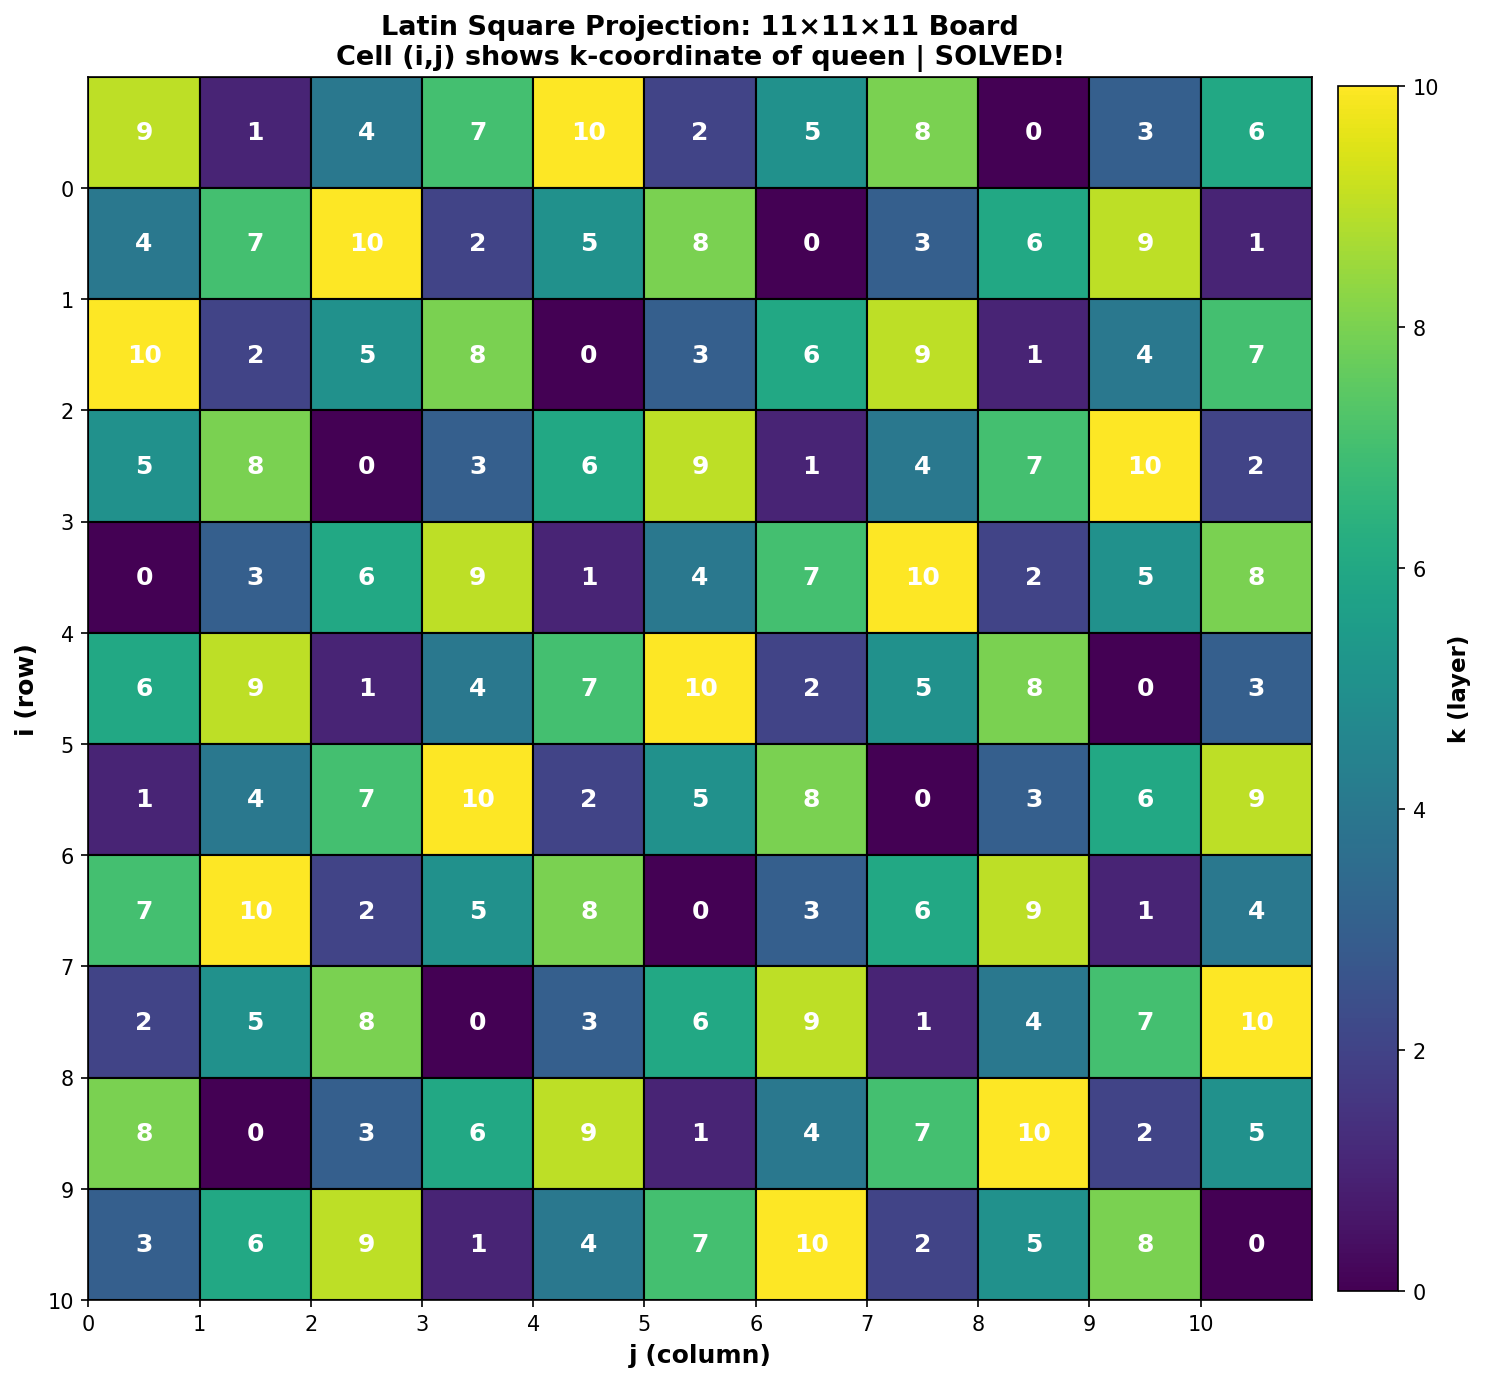
\includegraphics[width=\linewidth]{figures/solution-quadratic.png}
\caption{$g(x)=x^2$}
\end{subfigure}\hfill
\begin{subfigure}{0.48\linewidth}
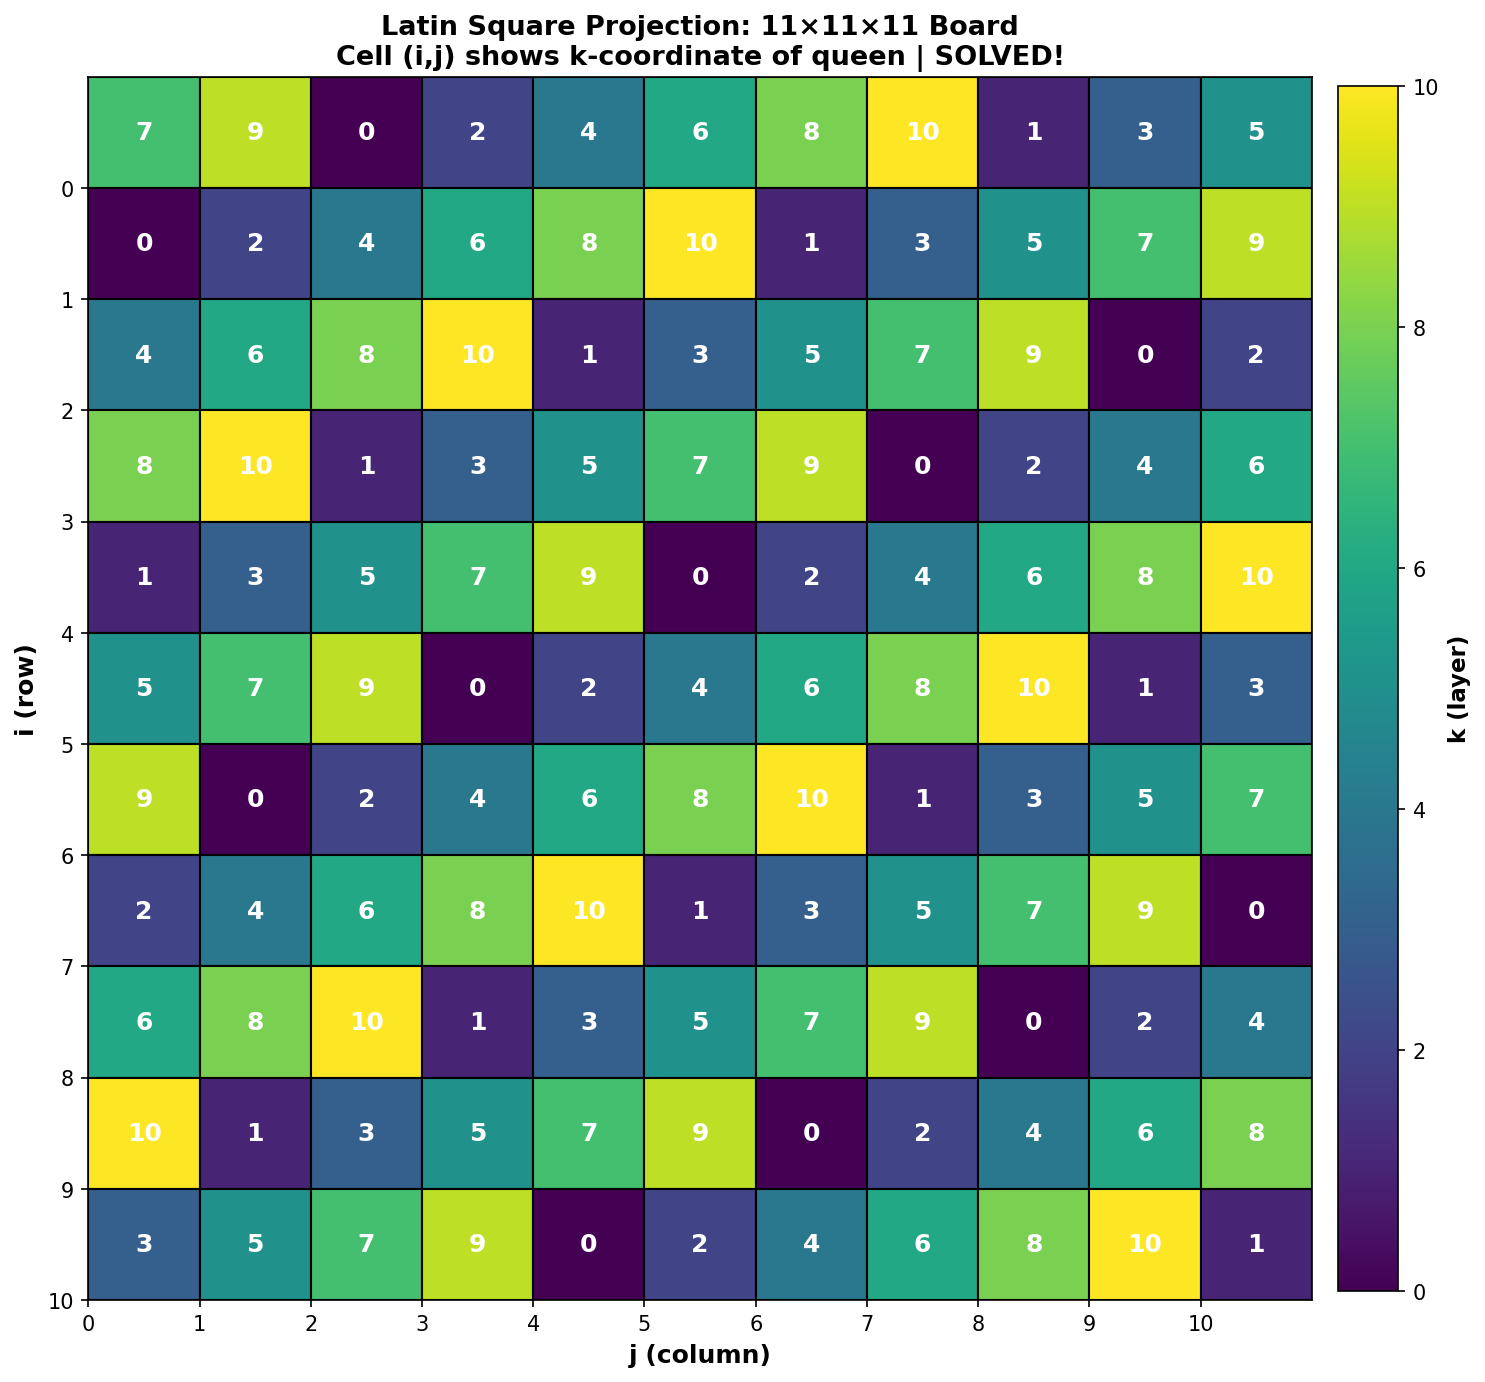
\includegraphics[width=\linewidth]{figures/solution-linear.png}
\caption{$g(x)=x$}
\end{subfigure}
\caption{Two distinct solutions for $N=11$.}
\label{fig:solutions}
\end{figure}

\subsection{Energy Evolution}
We examine energy evolution for $N=4$ to $N=11$, using linear cooling for $N\in\{4,5,6,11\}$ and geometric cooling for $N\in\{7,8,9,10\}$. Full results appear in Appendix~\ref{app:energy}; here we highlight the key cases $N=10$ and $N=11$ in Figure~\ref{fig:energy-main}.

The two cooling schedules produce distinct descent profiles. Linear cooling yields approximately linear curves with steady descent, while geometric cooling produces convex curves that drop rapidly early then flatten as high-temperature steps concentrate at the beginning. Both schedules converge to comparable final energies.

For $N\le10$, energy stabilizes at positive values, consistent with theoretical unsolvability. The final energy increases with board size, from around 21 for $N=4$ to 37 for $N=10$. For $N=11$, multiple runs reach zero energy, confirming existence of valid solutions. The individual trajectories diverge: some runs descend sharply to zero, while others plateau before finding the global minimum.

\begin{figure}[t]
\centering
\begin{subfigure}{0.48\linewidth}
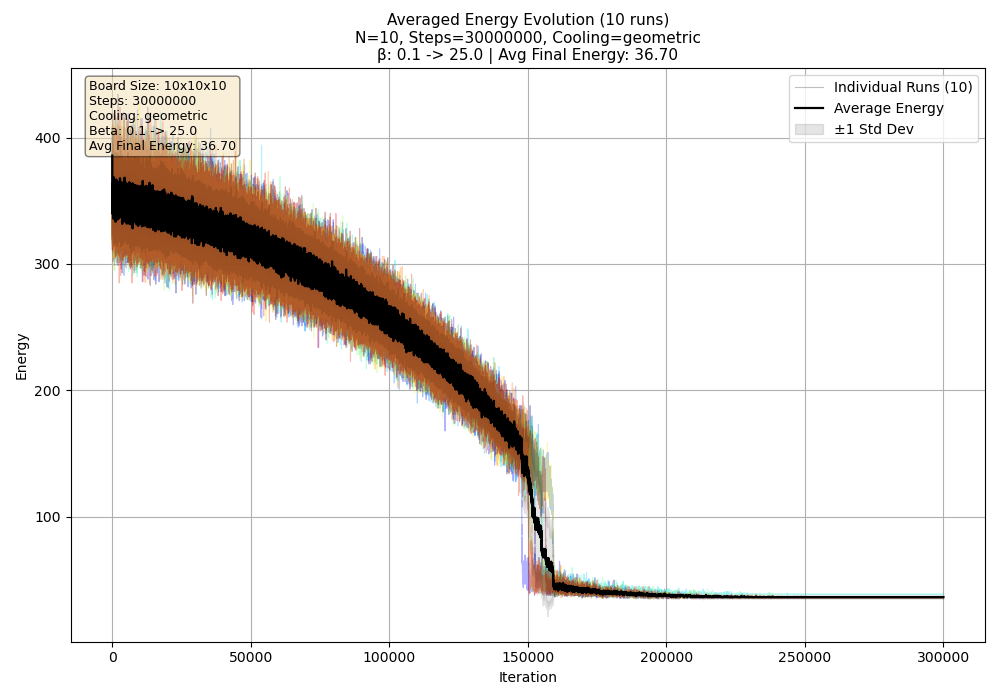
\includegraphics[width=\linewidth]{figures/energy-n10.png}
\caption{$N=10$ (geometric)}
\end{subfigure}\hfill
\begin{subfigure}{0.48\linewidth}
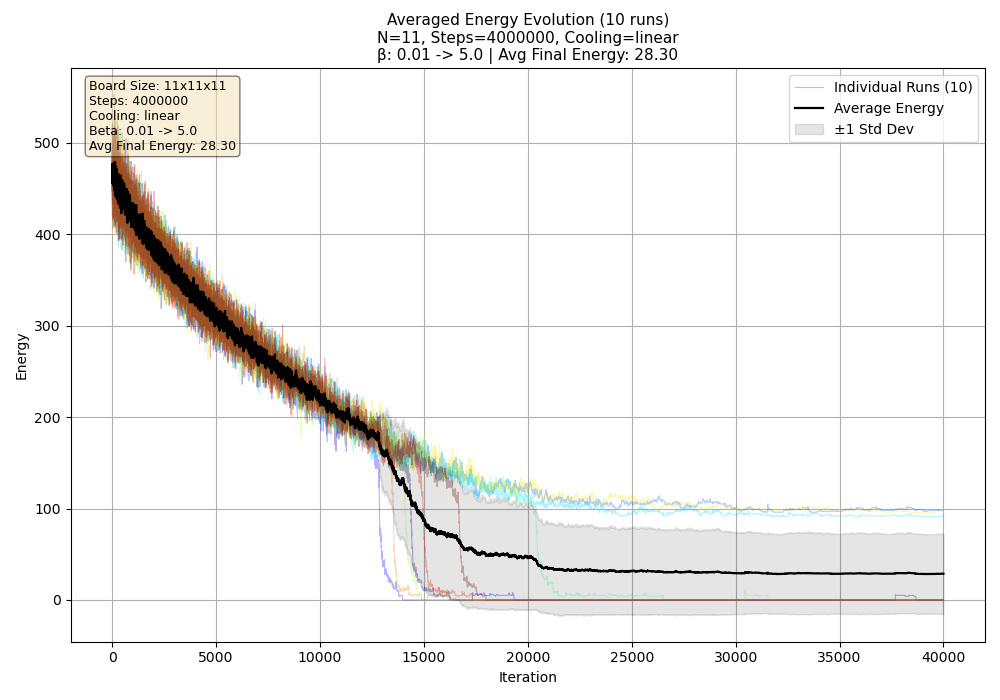
\includegraphics[width=\linewidth]{figures/energy-n11.png}
\caption{$N=11$ (linear)}
\end{subfigure}
\caption{Energy evolution for $N=10$ (unsolvable) and $N=11$ (solvable). Iteration axis scaled by $10^1$. Light: individual runs; dark: average. $\beta:0.1\to5$}
\label{fig:energy-main}
\end{figure}

\subsection{Effect of Annealing Schedule}
Simulated annealing gradually increases $\beta$ to balance exploration and exploitation. To assess whether this schedule is necessary, we compare runs with constant $\beta$ values ranging from 0.01 to 1000 for $N=11$.

As shown in Figure~\ref{fig:constant-beta}, low values ($\beta\le1$) accept too many uphill moves, causing the chain to oscillate at high energy without converging. High values ($\beta\ge10$) converge effectively to zero energy, suggesting that a greedy approach suffices for this problem size. Moreover, larger $\beta$ values yield faster convergence: $\beta=1000$ reaches zero energy in approximately 5000 iterations, compared to around 15000 for $\beta=10$. This behavior likely reflects a relatively benign energy landscape with few local minima. For larger $N$, the solution space grows and local minima proliferate, potentially requiring annealing to escape traps.

\begin{figure}[t]
\centering
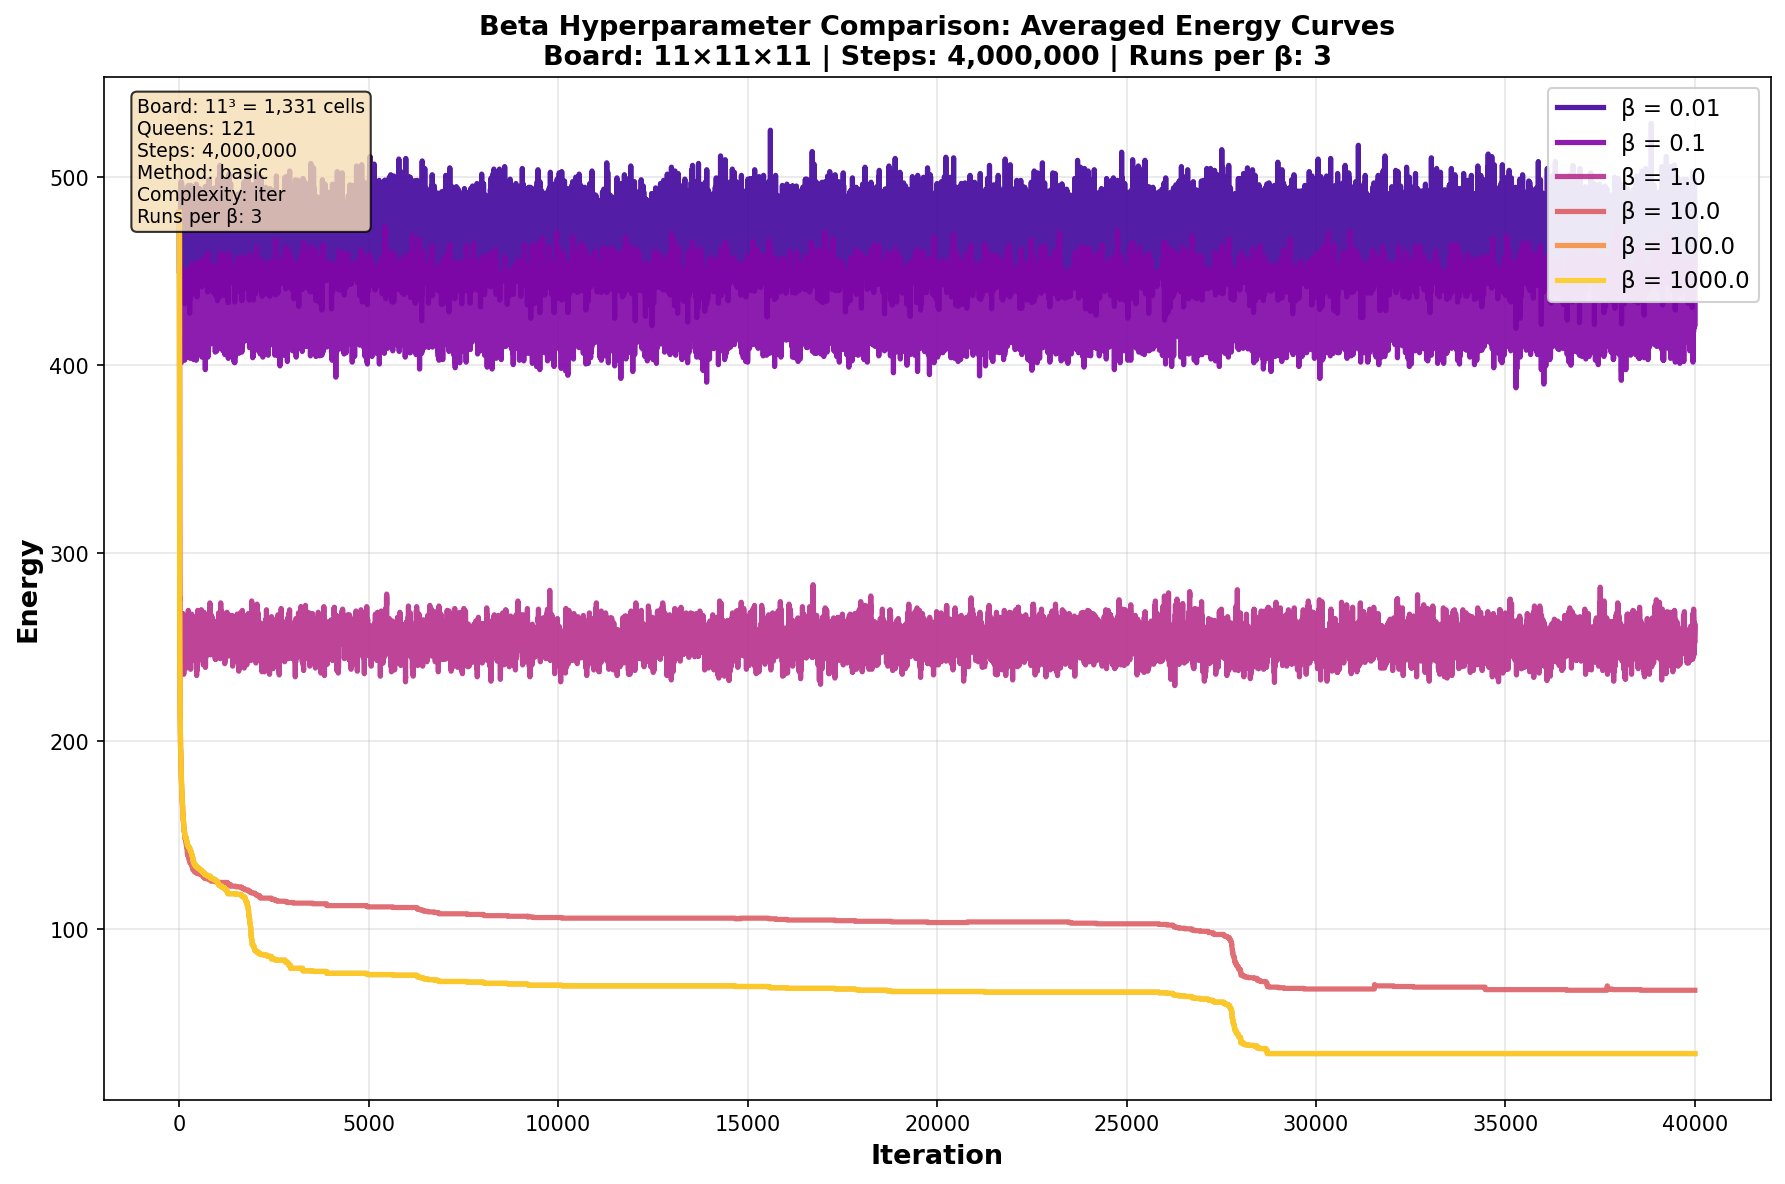
\includegraphics[width=\linewidth]{figures/constant-beta-comparison.png}
\caption{Energy evolution with constant $\beta$ for $N=11$. Low $\beta$ oscillates; high $\beta$ converges to zero.}
\label{fig:constant-beta}
\end{figure}

\subsection{Minimal Energy vs Board Size}
We examine how the minimal achievable energy varies with board size. Table~\ref{tab:minimal-energy} reports the best energy obtained across all runs for each $N$.

For $N\le10$, the algorithm converges to positive energy, with the minimum generally increasing with $N$ as the number of potential conflicts grows. The exception at $N=10$, which achieves lower energy than $N=8$ and $N=9$, may reflect variance across runs or favorable structure in the energy landscape. For $N=11$, the algorithm reaches zero energy, confirming the existence of a valid solution as predicted by $\gcd(11,210)=1$.

\begin{table}[h]
\centering
\begin{tabular}{c|rrrrrrrrr}
\hline
$N$&3&4&5&6&7&8&9&10&11\\
\hline
$J_{\min}$&13&21&32&41&50&53&55&36&\textbf{0}\\
\hline
\end{tabular}
\caption{Minimal energy achieved for each board size. Only $N=11$ reaches zero.}
\label{tab:minimal-energy}
\end{table}

\subsection{Favorable Values of $N$}
We identify which board sizes admit zero-energy configurations. Among all tested values, only $N=11$ achieves zero energy (Figure~\ref{fig:energy-main}), with a representative solution shown in Figure~\ref{fig:solutions}. This result aligns with the theoretical condition $\gcd(N,210)=1$: since 11 is coprime to 210, a solution is guaranteed to exist. Conversely, for $N=4$ to 10, all of which share common factors with 210, the algorithm converges to positive energy, empirically confirming their unsolvability.

\section{Conclusion}\label{sec:conclusion}
We have presented an MCMC approach to the three-dimensional $N^2$-queens problem, placing $N^2$ non-attacking queens on an $N\times N\times N$ board. Our formulation defines attack relations generalizing classical chess moves to three dimensions, introduces an energy function counting attacking pairs, and constructs a Metropolis-Hastings chain with provable correctness guarantees.

Experimental results across $N=3$ to $N=11$ confirm theoretical predictions: the algorithm converges to positive energy for unsolvable instances ($N\le10$) and successfully finds zero-energy configurations for $N=11$, consistent with the sufficient condition $\gcd(N,210)=1$. Our analysis of energy transformations reveals that only the linear function $g(x)=x$ reliably reaches global minima, while quadratic and logarithmic alternatives distort the energy landscape unfavorably. Surprisingly, for moderate $N$, constant high-$\beta$ schedules outperform simulated annealing, suggesting a relatively benign landscape with few local minima at these problem sizes.

Several directions remain for future work. Most promising is adopting the restricted state space formulation discussed in Section~\ref{sec:formulation}, which encodes configurations as functions $\kappa:\{0,\ldots,N-1\}^2\to\{0,\ldots,N-1\}$. This representation reduces the state space from $\binom{N^3}{N^2}$ to $N^{N^2}$, eliminates rook-type attacks along one axis by construction, and preserves all zero-energy solutions. The resulting efficiency gains would enable exploration of larger solvable values such as $N=13$, 17, or 19. Additionally, all $\beta$ tuning in this work was performed manually; systematic approaches such as grid search over initial and final $\beta$ values, or adaptive update rules, could further improve convergence. Other directions include informed proposal distributions targeting high-conflict queens and theoretical analysis of the energy landscape structure.

\begin{thebibliography}{1}
\bibitem[Kunt(2024)]{Kunt2024nQueensHigherDimensions}
Tim Kunt. The $n$-queens problem in higher dimensions, 2024. URL \url{https://arxiv.org/abs/2406.06260}.
\end{thebibliography}

\clearpage
\appendix
\section{Energy Evolution Plots}\label{app:energy}
Figure~\ref{fig:energy-all} presents energy evolution for all board sizes $N=4$ to $N=11$.

\begin{figure}[h]
\centering
\begin{subfigure}{0.48\linewidth}
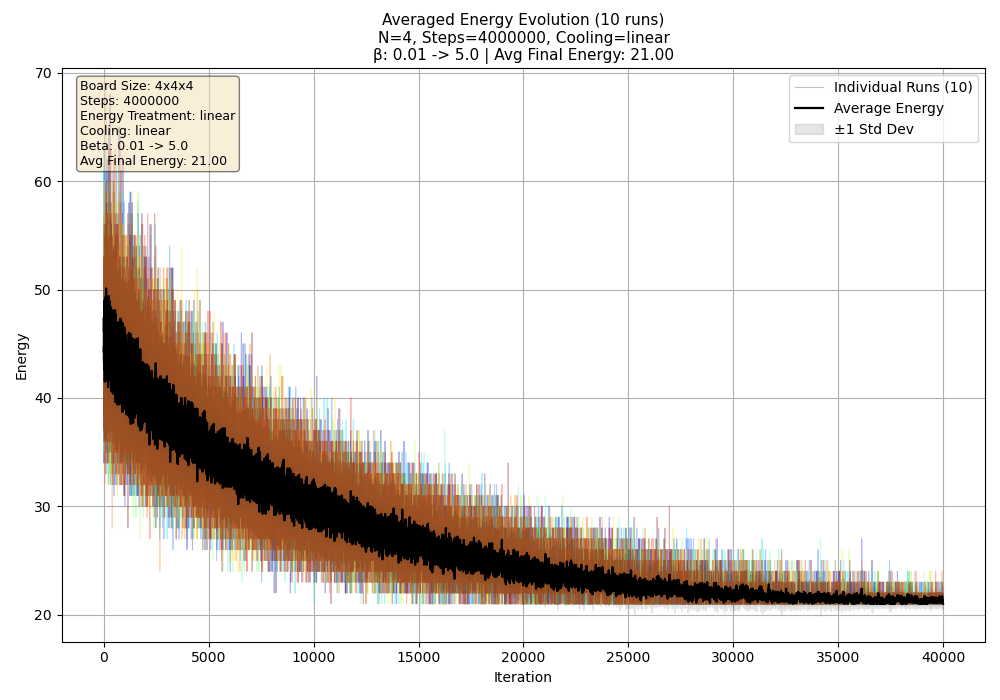
\includegraphics[width=\linewidth]{figures/energy-n4.png}
\caption{$N=4$ (linear)}
\end{subfigure}\hfill
\begin{subfigure}{0.48\linewidth}
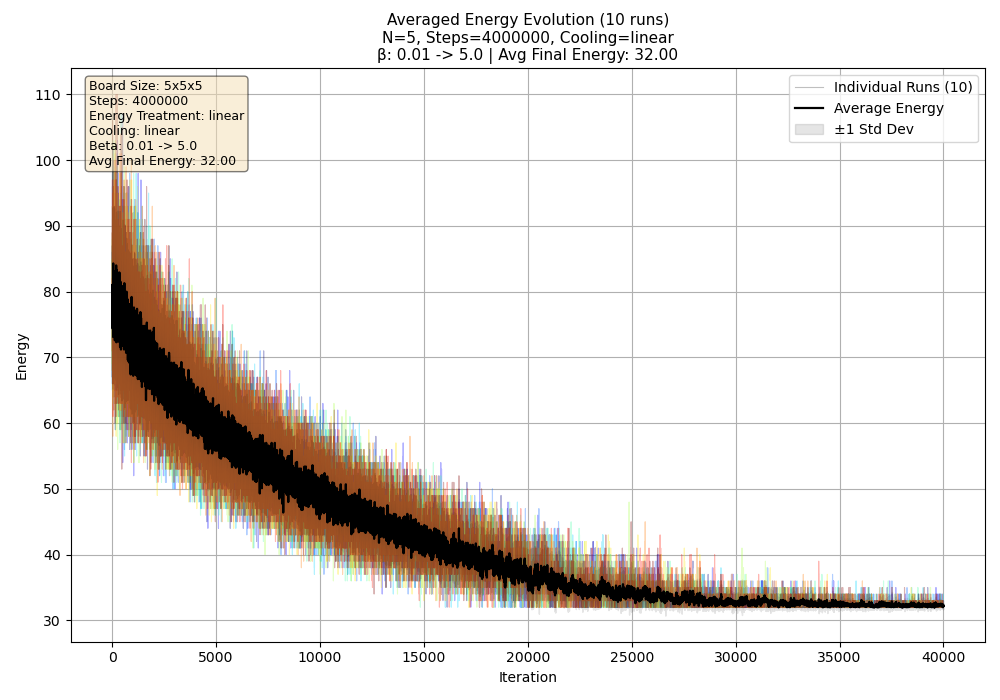
\includegraphics[width=\linewidth]{figures/energy-n5.png}
\caption{$N=5$ (linear)}
\end{subfigure}
\par\medskip
\begin{subfigure}{0.48\linewidth}
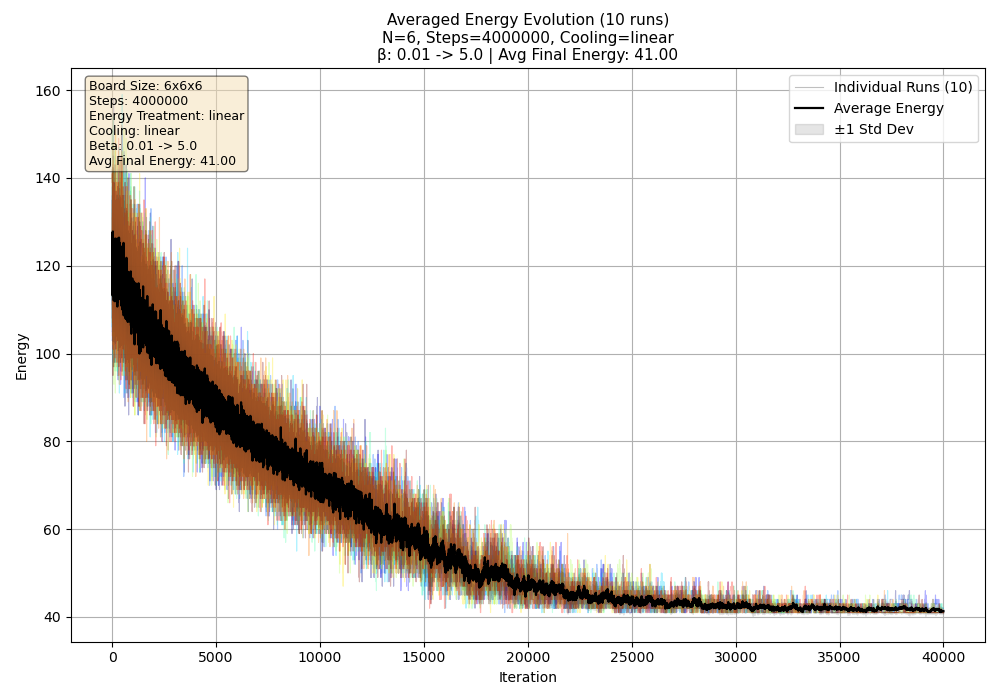
\includegraphics[width=\linewidth]{figures/energy-n6.png}
\caption{$N=6$ (linear)}
\end{subfigure}\hfill
\begin{subfigure}{0.48\linewidth}
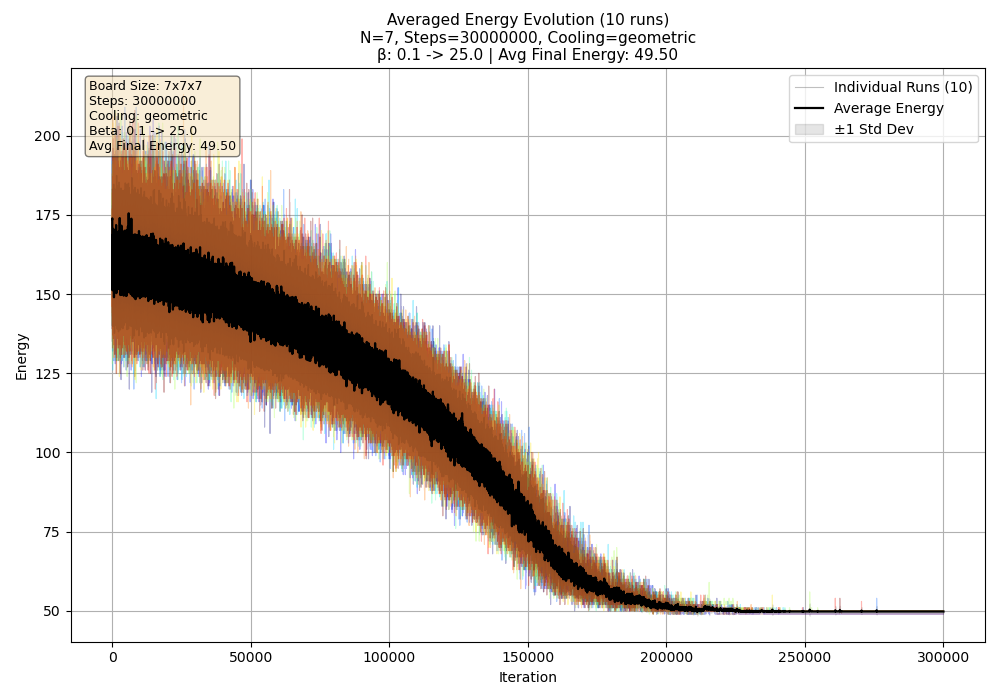
\includegraphics[width=\linewidth]{figures/energy-n7.png}
\caption{$N=7$ (geometric)}
\end{subfigure}
\par\medskip
\begin{subfigure}{0.48\linewidth}
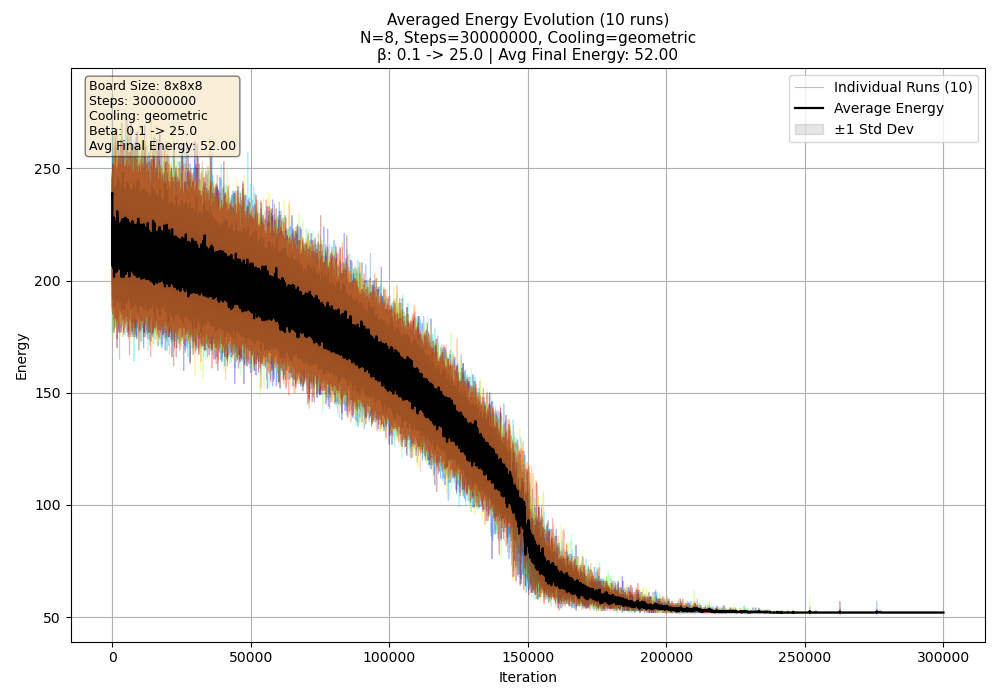
\includegraphics[width=\linewidth]{figures/energy-n8.png}
\caption{$N=8$ (geometric)}
\end{subfigure}\hfill
\begin{subfigure}{0.48\linewidth}
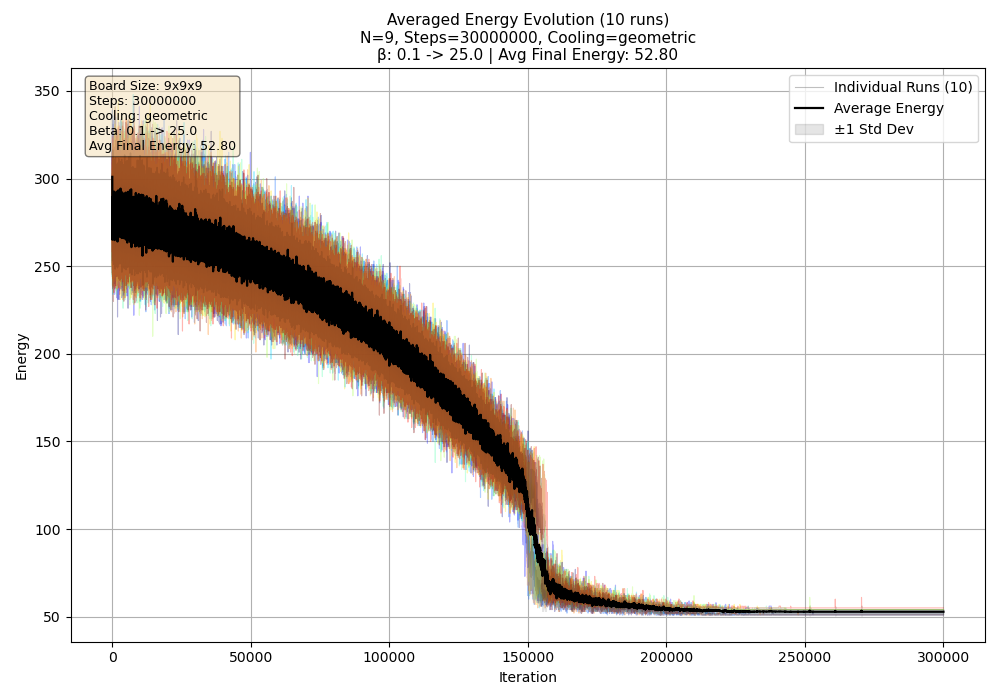
\includegraphics[width=\linewidth]{figures/energy-n9.png}
\caption{$N=9$ (geometric)}
\end{subfigure}
\par\medskip
\begin{subfigure}{0.48\linewidth}
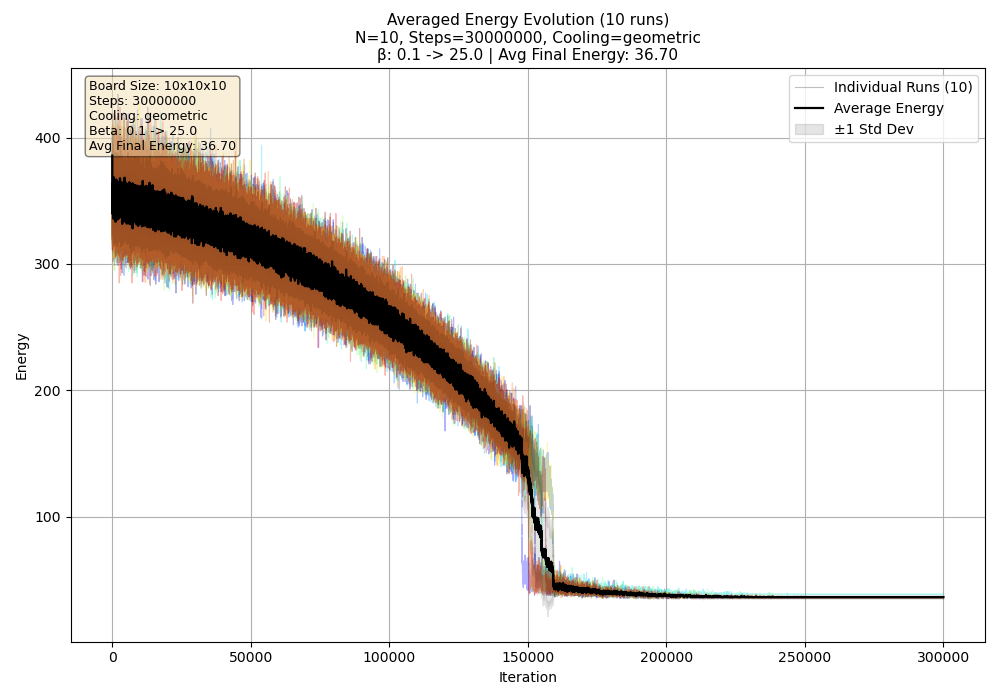
\includegraphics[width=\linewidth]{figures/energy-n10.png}
\caption{$N=10$ (geometric)}
\end{subfigure}\hfill
\begin{subfigure}{0.48\linewidth}
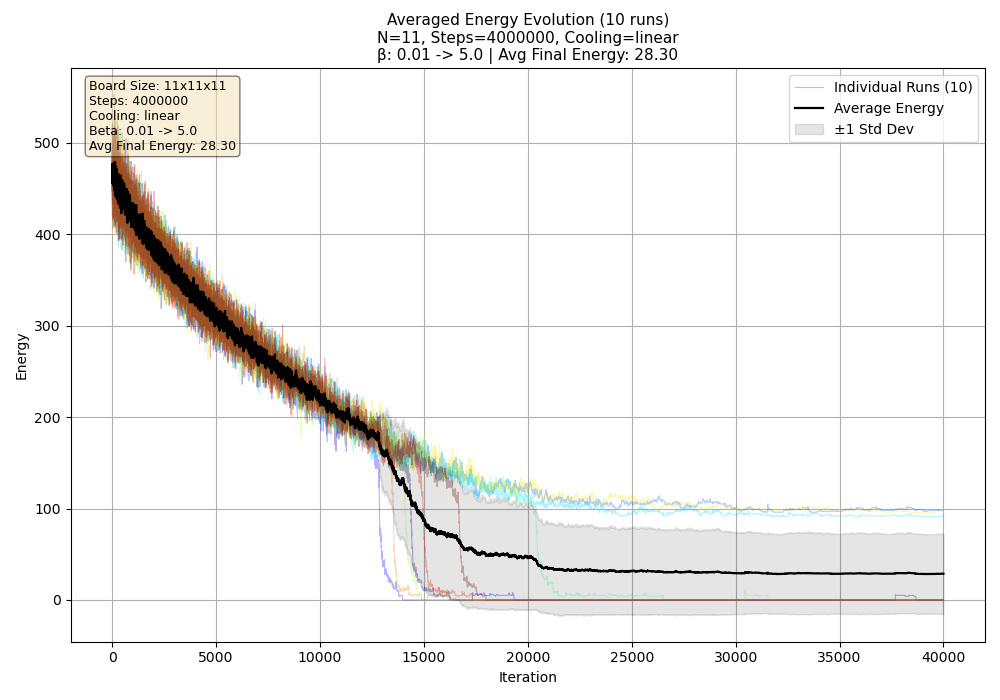
\includegraphics[width=\linewidth]{figures/energy-n11.png}
\caption{$N=11$ (linear)}
\end{subfigure}
\caption{Energy evolution for $N=4$ to $N=11$. Linear cooling for $N\in\{4,5,6,11\}$; geometric for $N\in\{7,8,9,10\}$. Iteration axis scaled by $10^1$. Light: individual runs; dark: average. $\beta:0.1\to5$.}
\label{fig:energy-all}
\end{figure}
\end{document}
